%%%%%%%%%%%%%%%%%%%%%%%%%%%%%%%%%%%%%%%%%%%%%%%%%%%%%%%%%%%%%%%%%%%%%%%%%%%%%%%%
% Homework 6 Solutions - C191A: Introduction to Quantum Computing
% Provided by Gemini
%%%%%%%%%%%%%%%%%%%%%%%%%%%%%%%%%%%%%%%%%%%%%%%%%%%%%%%%%%%%%%%%%%%%%%%%%%%%%%%%
\documentclass[11pt]{article}

% PACKAGES
\usepackage[a4paper, margin=1in]{geometry}
\usepackage{amsmath, amssymb, amsfonts}
\usepackage{graphicx}
\usepackage{tikz}

% CUSTOM COMMANDS for Quantum Mechanics
\newcommand{\ket}[1]{\left|{#1}\right\rangle}
\newcommand{\bra}[1]{\left\langle{#1}\right|}
\newcommand{\braket}[2]{\left\langle{#1}\middle|{#2}\right\rangle}
\newcommand{\matrixel}[3]{\left\langle{#1}\middle|{#2}\middle|{#3}\right\rangle}
\newcommand{\abs}[1]{\left|{#1}\right|}

% DOCUMENT INFO
\title{Homework 6 \\ Fall 2025}
\author{Xiaoyang Zheng}
\date{\today}

\begin{document}

\maketitle

\hrule\vspace{1em}

\section*{Problem 1: Phase Estimation}

\subsection*{1.1: What is $U^k|+\rangle$ written in the computational basis?}

$$
U^k \ket{+} = U^k \left( \frac{1}{\sqrt{2}}(\ket{0} + \ket{1}) \right)
= \frac{1}{\sqrt{2}} (U^k\ket{0} + U^k\ket{1}) = \frac{1}{\sqrt{2}} (\ket{0} + e^{ik\theta}\ket{1})
$$


\subsection*{1.2: Identify two projective measurements $\langle m_c|$ and $\langle m_s|$}

State after the operation: $\ket{\psi_k} = U^k\ket{+} = \frac{1}{\sqrt{2}} (\ket{0} + e^{ik\theta}\ket{1})$

For the first measurement,expect: $|\braket{m_c}{\psi_k}|^2 = \frac{1+\cos(k\theta)}{2}$

Projecting onto $\ket{+}$ state:
$$
\braket{+}{\psi_k} = \frac{1}{\sqrt{2}}(\bra{0}+\bra{1}) \cdot \frac{1}{\sqrt{2}}(\ket{0} + e^{ik\theta}\ket{1}) = \frac{1}{2}(1 + e^{ik\theta})
$$
The probability is:
$$
|\braket{+}{\psi_k}|^2 = \abs{\frac{1}{2}(1 + \cos(k\theta) + i\sin(k\theta))}^2= \frac{1}{4}(2+2\cos(k\theta)) = \frac{1+\cos(k\theta)}{2}
$$
So: $\bra{m_c} = \bra{+} = \frac{1}{\sqrt{2}}(\bra{0}+\bra{1})$.

For the second measurement, expect: $|\braket{m_s}{\psi_k}|^2 = \frac{1+\sin(k\theta)}{2}$

Projecting onto $\ket{+i} = \frac{1}{\sqrt{2}}(\ket{0} + i\ket{1})$

The corresponding bra is $\bra{+i} = \frac{1}{\sqrt{2}}(\bra{0} - i\bra{1})$.
$$
\braket{+i}{\psi_k} = \frac{1}{\sqrt{2}}(\bra{0}-i\bra{1}) \cdot \frac{1}{\sqrt{2}}(\ket{0} + e^{ik\theta}\ket{1}) = \frac{1}{2}(1 - ie^{ik\theta})
$$
The probability is the squared magnitude:
$$
|\braket{+i}{\psi_k}|^2 = \abs{\frac{1}{2}(1 - i(\cos(k\theta) + i\sin(k\theta)))}^2 = \frac{1}{4}(1+2\sin(k\theta)+\sin^2(k\theta)+\cos^2(k\theta)) = \frac{1+\sin(k\theta)}{2}
$$
So, $\bra{m_s} = \bra{+i} = \frac{1}{\sqrt{2}}(\bra{0}-i\bra{1})$.
$$
\bra{m_c} = \bra{+} \quad \text{and} \quad \bra{m_s} = \bra{+i}
$$

\subsection*{1.3: How can you estimate $\theta$ for $k=1$? Why can we not just use a single measurement?}
For $k=1$,: Caculate probability $p_c = |\braket{m_c}{\psi_1}|^2$ and $p_s = |\braket{m_s}{\psi_1}|^2$ 
$$
p_c = \frac{1+\cos(\theta)}{2} \implies \cos(\theta) = 2p_c - 1
$$
$$
p_s = \frac{1+\sin(\theta)}{2} \implies \sin(\theta) = 2p_s - 1
$$
Estimated $\cos(\theta)$ and $\sin(\theta)$, the angle $\theta \in [0, 2\pi)$ is determined using : $\theta = \operatorname{atan2}(2p_s - 1, 2p_c - 1)$.

\textbf{We cannot use a single measurement} because:
\begin{itemize}
    \item If we only measure $\cos(\theta)$, we cannot distinguish between $\theta$ and $2\pi - \theta$, as $\cos(\theta) = \cos(2\pi-\theta)$.
    \item If we only measure $\sin(\theta)$, we cannot distinguish between $\theta$ and $\pi - \theta$, as $\sin(\theta) = \sin(\pi-\theta)$.
\end{itemize}

\subsection*{1.4: What problems arise when trying to estimate $\theta$ for $k>1$?}
For $k>1$, we measure $\cos(k\theta)$ and $\sin(k\theta)$, giving $k\theta \pmod{2\pi}$. Then:
$$ k\theta = \phi + 2\pi m \implies \theta = \frac{\phi}{k} + \frac{2\pi m}{k} $$
There are $k$ possible values ($m = 0, \ldots, k-1$) that produce unique $\theta \in [0, 2\pi)$. We cannot determine $m$ from measurement alone.

\subsection*{1.5: How can you use information you gain from taking measurements at $k=1$ to solve this problem at $k=2$?}
\begin{enumerate}
    \item For $k=1$: Get estimate $\hat{\theta}_1$ (unambiguous).
    \item For $k=2$: Get $\phi_2 = 2\theta \pmod{2\pi}$, giving two candidates: $\frac{\phi_2}{2}$ or $\frac{\phi_2}{2}+\pi$.
    \item Choose the candidate closer to $\hat{\theta}_1$.
\end{enumerate}

\hrule\vspace{1em}

\section*{Problem 2: Grover's Algorithm on 2 qubits}

\subsection*{2.1: Write out the 2-qubit Oracle unitary $U_f$ as a $4 \times 4$ matrix.}
Oracle: $U_f\ket{x} = (-1)^{f(x)}\ket{x}$, where $f(11)=1$ and $f(x)=0$ otherwise. Basis: $\{\ket{00}, \ket{01}, \ket{10}, \ket{11}\}$.
$$
U_f = \begin{pmatrix} 1 & 0 & 0 & 0 \\ 0 & 1 & 0 & 0 \\ 0 & 0 & 1 & 0 \\ 0 & 0 & 0 & -1 \end{pmatrix}
$$
This is a Controlled-Z gate.

\subsection*{2.2: Write $|u\rangle$ and how to generate it.}
Equal superposition for 2 qubits ($N=4$):
$$
\ket{u} = \frac{1}{2}(\ket{00} + \ket{01} + \ket{10} + \ket{11})
$$
Generated by: $(H \otimes H) \ket{00}$

\subsection*{2.3: Draw the equal weight superposition $|u\rangle$ on a diagram.}
State space basis: marked state $\ket{a} = \ket{11}$ and unmarked superposition $\ket{e} = \frac{1}{\sqrt{3}}(\ket{00} + \ket{01} + \ket{10})$.
$$
\ket{u} = \frac{\sqrt{3}}{2}\ket{e} + \frac{1}{2}\ket{a}
$$
Angle with $\ket{e}$ axis: $\theta = \arcsin(1/2) = \pi/6$.

\begin{center}
\begin{tikzpicture}[scale=2.5]
    % Axes
    \draw[->, gray] (-1.1,0) -- (1.1,0) node[right, black] {$\ket{e}$};
    \draw[->, gray] (0,-0.2) -- (0,1.1) node[above, black] {$\ket{a}$};
    \node at (0,0) [below left] {$O$};
    % Vector |u>
    \draw[->, thick, blue] (0,0) -- (0.866, 0.5) node[above right, blue] {$\ket{u}$};
    % Angle theta
    \draw[->, gray] (0.4,0) arc (0:30:0.4);
    \node at (0.45, 0.1) {$\theta$};
\end{tikzpicture}
\end{center}

\subsection*{2.4: What is the angle $\theta$ between the vectors $|e\rangle$ and $|u\rangle$?}
$$
\cos(\theta) = \braket{u}{e} = \left(\frac{\sqrt{3}}{2}\bra{e} + \frac{1}{2}\bra{a}\right) \ket{e} = \frac{\sqrt{3}}{2}
$$
$$
\theta = \arccos\left(\frac{\sqrt{3}}{2}\right) = \frac{\pi}{6}
$$

\subsection*{2.5: Action of the Oracle $U_f$ on $|u\rangle$.}
$$ U_f\ket{a} = -\ket{a}, \quad U_f\ket{e} = \ket{e} $$
$$
U_f\ket{u} = U_f\left(\frac{\sqrt{3}}{2}\ket{e} + \frac{1}{2}\ket{a}\right) = \frac{\sqrt{3}}{2}\ket{e} + \frac{1}{2}(-\ket{a}) = \frac{\sqrt{3}}{2}\ket{e} - \frac{1}{2}\ket{a}
$$
Geometric: reflection about $\ket{e}$ axis.

\subsection*{2.6: Geometric interpretation of the action of $U_u$.}
$U_u = I - 2\ket{u}\bra{u}$ is a reflection operator.
$$
U_u\ket{u} = \ket{u} - 2\ket{u}\braket{u}{u} = -\ket{u}
$$
$$
U_u\ket{u^\perp} = \ket{u^\perp} - 2\ket{u}\braket{u}{u^\perp} = \ket{u^\perp}
$$
Geometric: reflection about the hyperplane perpendicular to $\ket{u}$.

\subsection*{2.7: Apply one iteration of Grover's algorithm.}
\begin{enumerate}
    \item Start: $\ket{u} = \frac{\sqrt{3}}{2}\ket{e} + \frac{1}{2}\ket{a}$
    \item Apply $U_f$: $\ket{u'} = \frac{\sqrt{3}}{2}\ket{e} - \frac{1}{2}\ket{a}$
    \item Apply $U_u$: $\ket{u''} = \ket{u'} - 2\ket{u}\braket{u}{u'}$
    
    $$ \braket{u}{u'} = \frac{3}{4} - \frac{1}{4} = \frac{1}{2} $$
    $$ \ket{u''} = \ket{u'} - \ket{u} = \left(\frac{\sqrt{3}}{2}\ket{e} - \frac{1}{2}\ket{a}\right) - \left(\frac{\sqrt{3}}{2}\ket{e} + \frac{1}{2}\ket{a}\right) = -\ket{a} $$
\end{enumerate}
Final state: $-\ket{a}$. Measurement yields '11' with 100\% probability.

\begin{center}
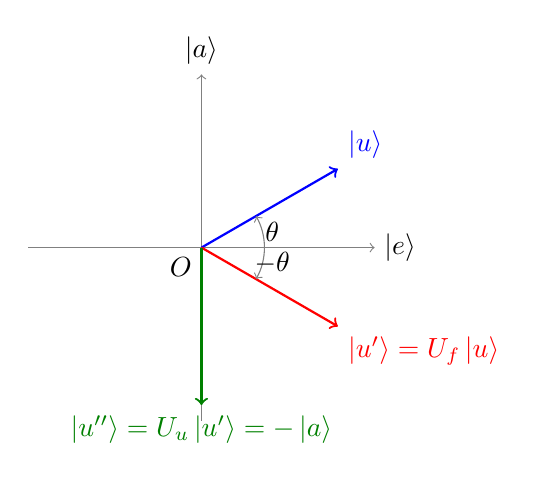
\begin{tikzpicture}[scale=2]
    % Axes
    \draw[->, gray] (-1.1,0) -- (1.1,0) node[right, black] {$\ket{e}$};
    \draw[->, gray] (0,-1.1) -- (0,1.1) node[above, black] {$\ket{a}$};
    \node at (0,0) [below left] {$O$};
    % Vectors
    \draw[->, thick, blue] (0,0) -- (0.866, 0.5) node[above right] {$\ket{u}$};
    \draw[->, thick, red] (0,0) -- (0.866, -0.5) node[below right] {$\ket{u'} = U_f\ket{u}$};
    \draw[->, thick, green!50!black] (0,0) -- (0, -1) node[below] {$\ket{u''} = U_u\ket{u'} = -\ket{a}$};
    % Angles and labels
    \draw[->, gray] (0.4,0) arc (0:30:0.4);
    \node at (0.45, 0.1) {$\theta$};
    \draw[->, gray] (0.4,0) arc (0:-30:0.4);
    \node at (0.45, -0.1) {$-\theta$};
\end{tikzpicture}
\end{center}

\vspace{2em}
\hrule
\vspace{0.5em}
\noindent\textit{Note: All TikZ diagrams in this document were generated by Gemini 2.5 Pro from hand-drawn sketches.}

\end{document}